\documentclass[../masters.tex]{subfiles}

\begin{document}
\graphicspath{{./imgs/}{../imgs/}} %look for images

\section{Introduction}
Insert the introduction.

\section{Background Literature}
Insert lit background

\subsection{Probability Theory}
The calculus of Probability Theory was developed by Fermat and Pascal in order to better understand the problems introduced by uncertainty in gambling. From this dubious genesis a rich and incredibly powerful field has developed. We start our brief introduction of probability theory by restating Kolmogorov's three probability axioms - these axioms underpin the entire theory of probability.

Let the set $\Omega$ be the universe of possible events, also called the event space; that is, if we are uncertain about which of a number of possibilities are true then we let $\Omega$ represent all of them collectively. Let $P$ be some real valued function which satisfies the three axioms stated below.
\begin{ax}
$P(\Omega) = 1$. The probability of any event in $\Omega$ occurring is 1.
\end{ax}
\begin{ax}
$\forall \alpha \in \Omega,~P(\alpha) \geq 0$. The probability of any event in $\Omega$ occurring is non-negative. 
\end{ax}
\begin{ax}
$\forall \alpha, \beta \in \Omega,\text{ if } \alpha \cap \beta = \emptyset \text{ then } P(\alpha \cup \beta) = P(\alpha) + P(\beta)$. The probability of two mutually disjoint events in $\Omega$ occurring is equal to the sum of their probabilities.
\end{ax}
A function $P$ which satisfies these three axioms is known as a probability function. Based on these three axioms we are able to extend the theory to Theorem \ref{thrm_prob_union_intersect}.
\begin{thrm}
$\forall \alpha, \beta \in \Omega, P(\alpha \cup \beta) = P(\alpha) + P(\beta) + P(\alpha \cap \beta)$. The probability of two events occurring in $\Omega$ is equal to the sum of their probabilities less the probability of both occurring simultaneously.
\label{thrm_prob_union_intersect}
\end{thrm}

We now make precise what we mean by random variables: a random variable is a non-deterministic variable which is characterised by some uncertainty in its measurement. Semantically we indicate a specific value taken on by the random variable $X$ as $X=x$ or just denote it $x$. Thus the function $P(X=x)=P(x) \in \mathbb{R}$ indicates the probability of event $x$ occurring with respect to the random variable $X$. We denote $P(X)$ as the probability function of the random variable $X$.

Before we proceed let us briefly discuss how we can interpret the function $P$ for any random variable $X$. If $P(X=x)=1$ we are certain of event $x$ occurring, i.e. $X$ will only take on the value $x$. If $P(x)=0$ we are certain that event $x$ will not occur, i.e. $X$ will never take on the value $x$. Thus our certainty of event $x$ occurring is reflected by the magnitude of $P(x)$. Attempting to make the statement ``our certainty of event $x$ occurring" more precise leads us to two different physical interpretations of $P(x)$. The first is the frequentist interpretation: to the frequentist a probability is a long term average of the observations of event $x$ occurring in the event space. While this interpretation is satisfying if one deals with something which is easily measured e.g. the probability of a fair die rolling a 6, it fails to explain statements like: ``the probability of it raining tomorrow is 50\%". The reason the last statement is problematic is because the time span is ill defined. If we rather understand probabilities to mean subjective degrees of belief in event $x$ occurring this is no longer a problem. To ensure that these subjective beliefs are rational can be problematic. One way to ensure this is by requiring that if the probabilities were used in a betting game it is impossible to exploit them to one's advantage (or disadvantage). If this is possible then there is no difference between the interpretations described above. 

We will deal extensively with joint and marginal probability distributions. Consider the random variables $X$ and $Y$. The marginal probability distribution of $X$ is the function $P(X)$ and describes the probabilities of events involving only the variable $X$. The joint probability distribution of $X$ and $Y$ is the function $P(X,Y) = P(X \cup Y)$ and describes the union of the probability space of $X$ and $Y$. We introduce, without proof, Theorem \ref{thrm_marg}.
\begin{thrm}
\textbf{Marginalisation} $\sum_x P(x) = 1$ and $P(Y) = \sum_x P(x, Y)$. 
\label{thrm_marg}
\end{thrm}
We can reduce any joint distribution to a marginal one by summing (or integrating in the case of continuous random variables) out the appropriate variable. 

It is now necessary to define what we mean by conditional probability. Definition \ref{defn_cond_prob} makes precise how the knowledge that event $y$ has occurred alters our view of event $x$ occurring.  
\begin{defn}
\textbf{Conditional Probability} $P(X|Y) = \frac{P(X \cap Y)}{P(Y)}$ 
\label{defn_cond_prob}
\end{defn}
Note that if $P(Y) = 0$ then Definition \ref{defn_cond_prob} is undefined. Additionally, the function $P(\cdot|Y)$ is a probability function. We next define what we mean by a positive probability distribution in Definition \ref{defn_pos_distr}.
\begin{defn}
A probability distribution is positive if $P(x) > 0~\forall~x \in X$.
\label{defn_pos_distr}
\end{defn}
Clearly undefined conditional probabilities are not a problem in the setting of positive probability distributions. We also define the notion of independence, also sometimes called marginal independence, in Definition \ref{defn_indep}. 

As before, let $X$, $Y$ and $Z$ be random variables. Intuitively $X$ and $Y$ are independent if the outcome of $X$ does not influence the outcome of $Y$. It can be shown that independence is a symmetric property \cite{koller}.
\begin{defn}
\textbf{Independence} $X \indep Y \equiv P(X|Y) = P(X)$ 
\label{defn_indep}
\end{defn}
Generalising the concept of independence we define conditional independence by Definition \ref{defn_cond_indep}. Again this definition is symmetric \cite{koller}.
\begin{defn}
\textbf{Conditional Independence} $X \indep Y | Z \equiv P(X|Y,Z) = P(X|Z)$
\label{defn_cond_indep}
\end{defn}
Intuitively, if $X$ is conditionally independent of $Y$ given $Z$ then by observing $Z$ one gains nothing by observing $Y$. Clearly if $Z=\emptyset$ we have (marginal) independence. We also introduce Theorem \ref{thrm_chain_rule} which naturally leads us to the formulation of Bayes' Theorem (using Definition \ref{defn_cond_prob}) as shown in Theorem \ref{thrm_bayes}. 
\begin{thrm}
\label{thrm_chain_rule}  
\textbf{Chain Rule} Given the random variables $X_1$ and $X_2$ we have $P(X_1,X_2) = P(X_1)P(X_2|X_1)$. The generalisation to an arbitrary number of random variables is straightforward.
\end{thrm}
\begin{thrm}
\textbf{Bayes' Theorem} $P(X|Y) = \frac{P(Y|X)P(X)}{P(Y)}$
\label{thrm_bayes}
\end{thrm}
Under the Bayesian interpretation of Theorem \ref{thrm_bayes} we see that the posterior probability of some hypothesis $X$ given some evidence $Y$ being true is just the likelihood $P(Y|X)$ of the hypothesis supporting the evidence multiplied by the prior probability of the hypothesis $P(X)$ normalised by the prior of the evidence $P(Y)$. 

So far in our discussion we have implicitly only used discrete random variables, that is our probability space consisted out of a finite number of events or states. However, it is also necessary to make precise what we mean by a continuous random variable. A continuous random variable is characterised by a density function $f$ which assigns a weight to each possible value of the variable. Although the density function is itself not a probability function, if it satisfies $f(x) \geq 0~\forall x$ and $\int_{-\infty}^{+\infty} f(x)dx = 1$ then it can be used to generate one. The cumulative probability function $P(X \leq x)=\int_{x\prime \leq x}f(x\prime)dx\prime$ is one such example. 

To fully describe a system of random variables it is only necessary to know the joint distribution $P(X_1,X_2,...,X_n)$. Given the joint probability distribution inference (reasoning about the variables under uncertainty) may be performed. Common probabilistic queries involve computing posterior beliefs $P(X|Y=y)$ i.e. the probability function of $X$ given we have some information about $Y$. Other queries involve find the most probable explanation (called a MAP query) of some evidence i.e. finding $X$ which maximises $P(X, Y=y)$. More on this later. 

\subsubsection{Bayes' Theorem: Example}
This section will attempt to develop some intuition behind Theorem \ref{thrm_bayes}. We quote an excerpt from an article in the Economist \cite{eco1} and illustrate the use of Bayes' Rule in a canonical medical example \cite{korb}.

\textit{``The essence of the Bayesian approach is to provide a mathematical rule explaining how you should change your existing beliefs in the light of new evidence. In other words, it allows scientists to combine new data with their existing knowledge or expertise. The canonical example is to imagine that a precocious newborn observes his first sunset, and wonders whether the sun will rise again or not. He assigns equal prior probabilities to both possible outcomes, and represents this by placing one white and one black marble into a bag. The following day, when the sun rises, the child places another white marble in the bag. The probability that a marble plucked randomly from the bag will be white (ie, the child's degree of belief in future sunrises) has thus gone from a half to two-thirds. After sunrise the next day, the child adds another white marble, and the probability (and thus the degree of belief) goes from two-thirds to three-quarters. And so on. Gradually, the initial belief that the sun is just as likely as not to rise each morning is modified to become a near-certainty that the sun will always rise."}

Suppose you get tested for a certain disease. You know the disease affects 1 in 100 people. You also know that the false positive rate for the test is 20\% and the false negative rate for the test is is 10\%. Your test comes back positive. What are the chances of you having the disease given this information?

The information may be summarised as shown below. Let $D$ be a binary random variable indicating the presence of the disease and $\neg D$ indicates the absence. Let $T$ be a binary random variable indicating a positive test and $\neg T$ indicates a negative test. 
\begin{enumerate}
\item
The prior of the disease is $P(D) = 0.01$.
\item
False positive rate $P(T|\neg D) = 0.2 \implies P(\neg T|\neg D) = 0.8$.
\item
False negative rate $P(\neg T|D) = 0.1 \implies P(T|D) = 0.9$.
\end{enumerate}
A naive approach would conclude that since $P(T|D) = 0.9$ you are 90\% likely to have the disease. However, using Bayesian inference/reasoning we have: 
\begin{equation*}
\begin{aligned}
P(D|T) &= \frac{P(T|D)P(D)}{P(T)} \\
&=  \frac{P(T|D)P(D)}{\sum_D P(D,T)} \\
&= \frac{P(T|D)P(D)}{\sum_D P(D)P(T|D)} \\
& = \frac{0.9 \times 0.01}{0.01 \times 0.99 + 0.99 \times 0.2} \\
&\approx 0.04
\end{aligned}
\end{equation*}
Clearly there is a big difference between the naive approach and the Bayesian approach. The power of Bayesian inference lies in the ability to correctly reason about events under uncertainty given evidence.

\subsection{Graph Theory}
A graph, $G$, is a data structure consisting of a set of nodes $\chi$ and edges $\xi$. A pair of nodes $X_i, X_j \in \chi$ can be connected by an edge. We will only consider directed graphs in this dissertation. This implies that every edge in $\xi$ has a direction associated between the two nodes it connects i.e. $X_i \rightarrow X_j$ if there is an edge from $X_i$ to $X_j$.

We now define some basic concepts which we will rely upon to further describe the types of graphs we will consider.
\begin{defn}
\textbf{Directed Path} We say that the nodes $X_1, X_2, X_3,..., X_n \in \chi$ form a directed path if $X_i \rightarrow X_{i+1}$ for $1 \leq i \leq n-1$. 
\end{defn}
\begin{defn}
\textbf{Directed Cycle} A directed cycle is a non-singleton directed path which starts and ends at the same node.
\end{defn}
\begin{defn}
\textbf{Directed Acyclic Graph (DAG)} A graph $G$ is a DAG if it is directed and has no directed cycles.
\end{defn}
In this dissertation we will only concern ourselves with DAGs. Figure \ref{fig_dag} is an example of a DAG.
\begin{figure}[H] 
\centering
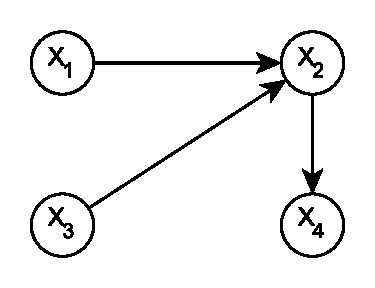
\includegraphics[scale=1.0]{dag.pdf}
\caption{Example of a Directed Acyclic Graph}
\label{fig_dag}
\end{figure}
Next we define some nomenclature to further describe the nodes of a graph $G$.
\begin{defn}
\textbf{Parents} We say that the set of nodes $\kappa \subset \chi$ are the parents of node $X_i$ if, for each node in $\kappa$, there exists an edge going to $X_i$.
\end{defn}
\begin{defn}
\textbf{Children} We say that the set of nodes $\tau \subset \chi$ are the children of node $X_i$ if, for each node in $\tau$, there exists an edge going from $X_i$ to that node.
\end{defn}
We also briefly define a structured approach to encoding a graph.
\begin{defn}
\textbf{Adjacency Matrix} For a graph $G$ with $n$ nodes, the adjacency matrix $A$ is an $n \times n$ matrix where $A_{ij} = 1$ if there is an edge from node $i$ to node $j$ and $A_{ij} = 0$ otherwise. 
\end{defn}
The adjacency matrix A for Figure \ref{fig_dag} is shown below:
\begin{equation*}
A = \begin{pmatrix}
0 & 1 & 0 & 0 \\
0 & 0 & 0 & 1 \\
0 & 1 & 0 & 0 \\
0 & 0 & 0 & 0
\end{pmatrix}
\end{equation*}

A detailed analysis of Graph Theory may be found in \cite{deo}.

\subsection{Probabilistic Graphical Models}
Probabilistic graphical models is the union between Probability Theory and Graph Theory. Consider why it is in general infeasible to determine an arbitrary joint probability distribution

\subsubsection{Bayesian Networks}

\subsubsection{d-separation}

\subsubsection{Dynamic Bayesian Networks}
Chapter 13 in Bishop! HMM and then KFs

\bibliographystyle{plain}
\bibliography{research}

\end{document}